\chapter{Fahrzeugprototyp}
\label{cha:Prototyp}
Das Gesamtkonzept für den Fahrzeugprototypen basiert auf der Vision eines \glqq Fahrzeuges als Leinwand\grqq{} (englisch: \glqq Car as a canvas\grqq{}). Das Zielbild dieser Vision ist ein Fahrzeug, das auf vollständige Weise sein Erscheinungsbild verändern kann. \\
Unter der übergeordneten Vision, das Fahrzeug als Leinwand zu betrachten, bildet das Gesamtkonzept des Prototypen einen möglichen ersten Schritt in Richtung der Vision.
\section{Gesamtkonzept}
Das Gesamtkonzept beruht im Kern auf digitaler Kunst im Fahrzeug. Kunden können unterschiedliche digitale Kunstinhalte, sogenannte Kollektionen, erwerben und diese Kollektionen in ihrem Fahrzeug aktivieren. Die Kollektionen bestehen aus mehreren inhaltlichen Bestandteilen, welche auf neuartigen und bestehenden Fahrzeugkomponenten im Fahrzeug dargestellt werden. Die Bestandteile werden als \glqq Collectible\grqq{} bezeichnet. Die Gesamtinszenierung der Kollektion wird durch bestimmte Trigger, wie zum Beispiel das Entriegeln der Türen, aktiviert. \\
Das Zusammenspiel zwischen den einzelnen Domänen im Kauf und der Verwaltung der Kollektion, beschreibt das Diagramm \ref{fig:gesamtkonzept}. Der Benutzer interagiert mit einer App. Durch den Kaufauftrag vom Benutzer in der App, wird die gewünschte Kollektion auf das Fahrzeug geladen. Durch Aktivierung der Kollektion in der App, wird die Kollektion dem Benutzer angezeigt. \\
\begin{figure}[hbt]
	\centering
	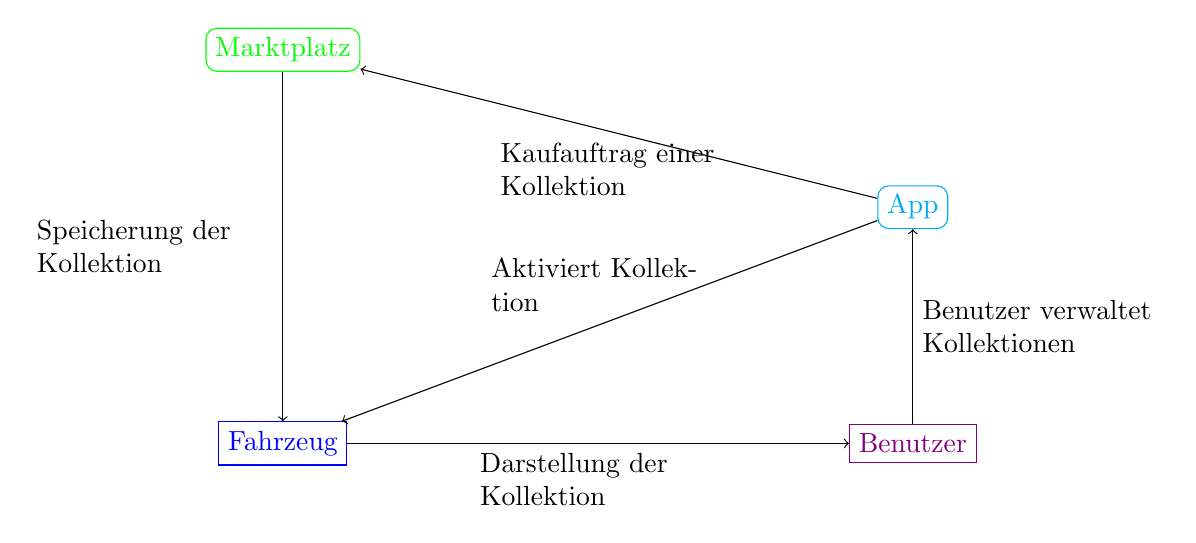
\begin{tikzpicture}[first style/.style={rectangle, draw, rounded corners, align=center}, steuer style/.style={draw, rectangle, align=center}, second/.style={text width=3cm}]
	\node[steuer style, blue] (S1) at (-3, 0) {Fahrzeug};
	\node[steuer style, violet] (S2) at (5, 0) {Benutzer};
	\node[first style, cyan] (S3) at (5, 3) {App};
	\node[first style, green] (S4) at (-3, 5) {Marktplatz};
	\draw[->] (S2) -- node[right, second] {Benutzer verwaltet Kollektionen} (S3);
	\draw[->] (S3) -- node[above, second] {Aktiviert Kollektion} (S1);
	\draw[->] (S1) -- node[below, second] {Darstellung der Kollektion} (S2);
	\draw[->] (S3) -- node[below, second] {Kaufauftrag einer Kollektion} (S4);
	\draw[->] (S4) -- node[left, second] {Speicherung der Kollektion} (S1);
\end{tikzpicture}
	\caption[Blockdiagramm Kollektionenverwaltung Gesamtkonzept]{Blockdiagramm Kollektionenverwaltung Gesamtkonzept}
	\label{fig:gesamtkonzept}
\end{figure}

Neben optischen Komponenten inszenieren haptische, olfaktorische und akustische Komponenten die Kollektionen. Dazu bilden Augmented Reality (AR\nomenclature{AR}{Augemented Reality}) Anwendungen weitere Collectibles der Kollektionen. Diese werden mit Hilfe einer eigenen App auf einem Mobiltelefon angezeigt.\\
Die App ist für den Besitzer das zentrale Bediensystem, in der unterschiedliche Aktionen auf den einzelnen Seiten verfügbar sind:
\begin{itemize}
	\item Kollektionen können auf digitalen Börsen gehandelt werden.
	\item Gekaufte Kollektionen können im Fahrzeug aktiviert werden oder durch AR auf dem Mobiltelefon gezeigt werden.
	\item Zusätzliche AR Collectibles zu den Kollektionen können auf dem Mobiltelefon gezeigt werden.
	\item Einzelne Collectibles der aktivierten Kollektion können deaktiviert werden.
	\item Über ein eigenes Profil kann mit anderen Besitzern von Kollektionen Bilder durch ein soziales Netzwerk ausgetauscht werden.
\end{itemize}
Im Gegensatz zu bisherigen Individualisierungsmöglichkeiten, wie zum Beispiel Ambientebeleuchtung oder LED-Scheinwerfer, können die Kollektionen in diesem Gesamtkonzept zum einen dynamisch ihre Inhalte verändern und zum anderen das gesamte Erscheinungsbild des Fahrzeugs ganzheitlich verändern. \\
\begin{figure}[hbt]
	\centering
	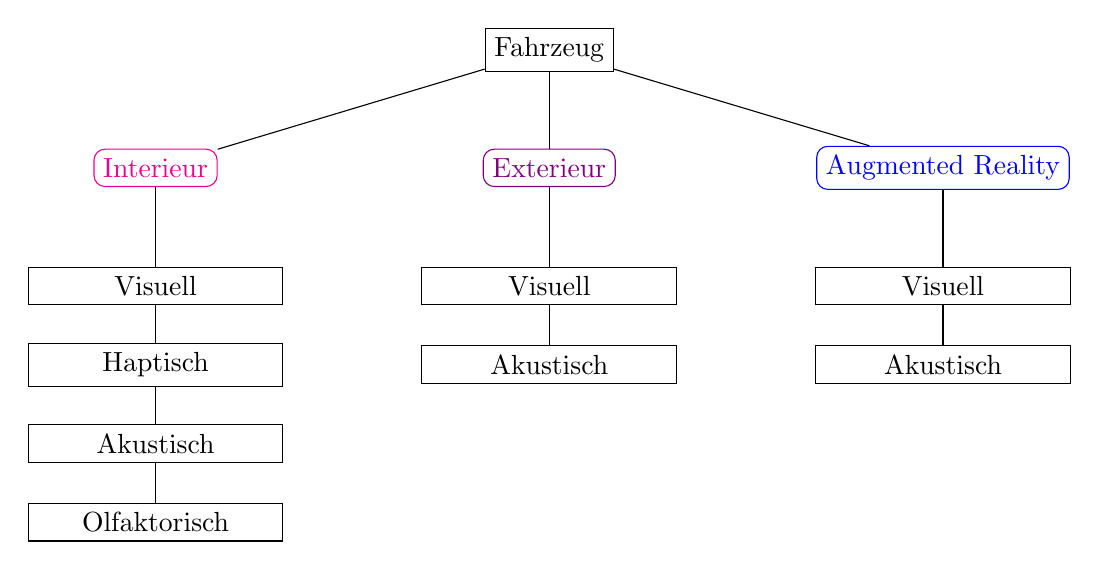
\begin{tikzpicture}[first style/.style={rectangle, draw, rounded corners, align=center}, steuer style/.style={draw, rectangle, align=center}, second/.style={draw, rectangle, align=center, text width=3cm}]
	\node[steuer style] (S1) at (0, 3) {Fahrzeug};
	\node[first style, magenta] (S2) at (-5, 1.5) {Interieur};
	\node[first style, violet] (S3) at (0, 1.5) {Exterieur};
	\node[first style, blue] (S4) at (5, 1.5) {Augmented Reality};
	\node[second] (S5) at (-5, 0) {Visuell};
	\node[second] (S6) at (-5, -1) {Haptisch};
	\node[second] (S7) at (-5, -2) {Akustisch};
	\node[second] (S8) at (-5, -3) {Olfaktorisch};
	\node[second] (S9) at (0, 0) {Visuell};
	\node[second] (S10) at (0, -1) {Akustisch};
	\node[second] (S11) at (5, 0) {Visuell};
	\node[second] (S12) at (5, -1) {Akustisch};
	\foreach \x in {2,...,4}
	\draw (S1) -- (S\x);
	\draw (S2) -- (S5);
	\draw (S5) -- (S6);
	\draw (S6) -- (S7);
	\draw (S7) -- (S8);
	\draw (S3) -- (S9);
	\draw (S9) -- (S10);
	\draw (S4) -- (S11);
	\draw (S11) -- (S12);
\end{tikzpicture}
	\caption[angesprochene Sinne nach Fahrzeugbereich]{angesprochene Sinne nach Fahrzeugbereich}
	\label{fig:sinneeinteilung}
\end{figure}

Das Diagramm \ref{fig:sinneeinteilung} teilt den drei Grundbereichen die verwendeten Sinneseindrücke zu. \\
Für das Gesamtkonzept wurden vier unterschiedliche Kollektionen erstellt. Die Collectibles zeigen je nach Trigger unterschiedliche Inhalte trotz gleicher Kollektion. In der folgenden Arbeit soll bei Berechnungen davon ausgegangen werden, dass ein Betrachter zehn Kollektionen besitzt. \\
Das Gesamtkonzept beinhaltet ein Ökosystem für den Handel und die Interaktion für Kollektionen als digitale Wertgegenstände.
%TODO Diagramm Ökosystem%
\section{Beschreibung}
Der Prototyp wurde unter den Leitlinien des Gesamtkonzeptes entwickelt. Die Basis des Prototypen bildet ein produziertes elektrisches Serienfahrzeug. An dem Fahrzeug wurden im Exterieur und Interieur entweder Teile ergänzt oder mit neuen Komponenten getauscht, die das Gesamtkonzept des Prototypen umsetzen. Die Serienfunktionen wurden zum größten Teil durch die Umbauten nicht beeinträchtigt.\\
Durch Zeit- und Budgetknappheit besitzt das Fahrzeug nicht alle Ideen des Gesamtkonzeptes. Bei den Hardware-Komponenten gibt es keine mit olfaktorischen Sinneseindrücken, sondern nur passende Düfte für die Kollektionen. Die App besitzt alle oben beschriebenen Funktionen zumindest als Schaubilder, aber hat nur die Auswahl und Steuerung der Kollektionen und AR Inhalte als Funktionen implementiert.
\section{Exterieur Komponenten}
Das Fahrzeug hat sowohl im Exterieur als auch im Interieur Komponenten verbaut. Zuerst werden die Komponenten im Exterieur und dann im Interieur vorgestellt. Die Komponenten wurden nach der verwendeten Technik und dem Ort benannt und nicht nach den Markennamen. Die Einteilung erfolgt nach der Betrachtungsweise innerhalb oder außerhalb des Fahrzeugs der Komponenten. Exterieur Komponenten werden von Beobachtern außerhalb des Fahrzeugs betrachtet. Interieur Komponenten entsprechend von innen.\\
%TODO Bild Komponenten Exterieur%
Im Exterieur sind dies:
\begin{itemize}
	\item ein E-Papier und ein durchgehendes LED-Streifen in der Frontschürze
	\item E-Papier über den beiden vorderen Radkästen
	\item LED-Streifen in allen vier Radkästen
	\item Videoprojektoren in den beiden Außenspiegel
	\item nach außen gerichtete Bildschirme in den hinteren Seitenfenstern
	\item ein LED-Streifen in der Heckleuchte und zwei kleine E-Papiere unterhalb der Heckleuchte
\end{itemize}
Im folgenden werden alle Exterieur Komponenten näher betrachtet:
\subsection{E-Papier in der Frontschürze}
Das E-Papier befindet sich hinter einer Scheibe mit einem Markenlogo in der Mitte der Fahrzeugfront und schließt an den Seiten über eine Abmaskierung auf die beiden Frontlichter ab. Das E-Papier bewirkt mit der Laminierung an der Scheibe einen räumlichen Effekt, wonach das Markenlogo vor dem E-Papier erscheint. \\
Auf dem E-Papier werden graphische Designs dargestellt, die Betrachter vor dem Auto sehen können. Dafür muss das Bild aus einer Entfernung von $ 1\,\mathrm{m} $ \nomenclature{m}{Meter} für den Betrachter scharf sein. \\
Das E-Papier hat ein Format von 16:9 und eine Auflösung von  $ 2560\,\mathrm{Pixel}/\mathrm{Zeile} \times 1440\,\mathrm{Zeilen} $, wovon ein Teil des Bildschirms am Rand durch eine Abmaskierung nicht sichtbar ist.
\subsection{LED-Streifen in der Frontschürze}
Der LED-Streifen ist dreiteilig aufgeteilt. Die zwei äußeren Teile befinden sich in den beiden Frontleuchten und schließen auf gleicher Höhe mit dem mittleren Streifen ab. Der mittlere Streifen befindet sich oberhalb des E-Papiers in der Frontschürze. \\
Auf dem Streifen können dynamische bunte Lichtsequenzen gezeigt werden. Für den Betrachter sollen die einzelnen LED aus einer Entfernung von $ 1\,\mathrm{m} $ nicht sichtbar sein und die Animationen flüssig erscheinen. Flüssig bedeutet, dass die Bildwiederholungsrate hoch genug ist, damit das Auge aus den einzelnen Bildern eine Bewegung erkennt. \\
Zusammen mit dem E-Papier in der Frontschürze bilden diese zwei
Komponenten die Darstellung der Kollektionen im Frontbereich. Der mittlere Teil besitzt 130 Bildpunkte und die äußeren Teile 101 Punkte. Mit insgesamt 332 LEDs lassen sich die einzelnen Punkte nicht erkennen.
\subsection{E-Papiere über den vorderen Radkästen}
Oberhalb der Radkästen befinden sich in einem ca. $ 20\,\mathrm{cm} $ breitem und $ 8\,\mathrm{cm} $ hohen Ausschnitt E-Papiere. An dieser Stelle befand sich vorher ein Emblem der Fahrzeugbezeichnung. \\
Die E-Papiere können genutzt werden, um den Namen der verwendeten Kollektion anzuzeigen. Dafür müssen Sie 20 Zeichen in einer Zeile mit einer Größe anzeigen, die ein Betrachter von mindestens $ 8\,\mathrm{m} $ Entfernung erkennt. \\
Die E-Papiere haben ein Format von 4:3 und eine Auflösung von $ 1600\,\mathrm{Pixel}/\mathrm{Zeile} \times 1200\,\mathrm{Zeilen} $, wodurch auch bei näherer Betrachtung noch ein scharfes Bild sichtbar ist.
\subsection{LED-Streifen in den Radkästen}
In allen vier Radkästen befinden sich LED-Streifen am äußeren Rand und strahlen durch eine Leiste in den Innenraum Radkasten auf den oberen Halbkreis des Reifenprofils. Der Betrachter sieht nicht den LED-Streifen, sondern nur das vom Reifen und Radkasten reflektierte Licht. \\
Pro Radkasten befinden sich 196 LEDs. Die Anzahl soll so hoch sein, dass die Beleuchtung ein homogenes Lichtbild gibt.
\subsection{Videoprojektoren in den Außenspiegeln}
In den Außenspiegeln wurde der Innenraum mit der Spiegelmechanik ausgebaut und Videoprojektoren eingebaut. Der nach unten ausgerichtete Videoprojektor bestrahlt die Flächen durch ein Loch an der Unterseite des Außenspiegels vor den vorderen Türen.
Durch den Videoprojektor können Videos auf dem Boden gezeigt werden. Der Betrachter soll hierbei aus einer kurzen Entfernung vom Fahrzeug das Bild scharf auf unterschiedlichen Böden und Lichtverhältnissen sehen können. \\
Die Videoprojektoren haben ein Format von 16:10 und eine Auflösung von $ 1280\,\mathrm{Pixel}/\mathrm{Zeile} \times 800\,\mathrm{Zeilen} $.
\subsection{Bildschirme in den hinteren Seitenfenstern}
In den hinteren Seitenfenstern befinden sich an den unbeweglichen Nebenscheiben, die mit einer Leiste von den beweglichen Hauptglasscheiben getrennt sind, Bildschirme. Diese können von außen betrachtet werden. Die Rückseite der Bildschirme ist von innen mit einer schwarzen Kunststoffverkleidung für die Passagiere abgedeckt.\\
Zusammen mit den LED-Streifen in den Radkästen und den Videoprojektoren in den Außenspiegeln bilden die Bildschirme in den Seitenfenstern die optische Darstellung der Kollektionen im Seitenbereich.
Die Bildschirme haben ein Verhältnis von 16:10 und eine Auflösung von $ 1280\,\mathrm{Pixel}/\mathrm{Zeile} \times 800 \,\mathrm{Zeilen} $, womit Betrachter aus $ 1\,\mathrm{m} $ Entfernung ein scharfes Bild sehen.
\subsection{LED-Streifen in der Heckleuchte}
In der Serienheckleuchte wurde das rote Leuchtband mit einem LED-Streifen getauscht. Der Streifen ist dreigeteilt mit dem mittleren Teil in der Heckklappe und den zwei äußeren Teilen im hinteren Kotflügel. \\
Der mittlere Streifen besitzt 219 LEDs und die äußeren Streifen 86 LEDs. Insgesamt sind in der Heckleuchte 391 LEDs verbaut.
\subsection{E-Papier in der Heckleuchte}
Direkt unterhalb der Heckleuchten sind zwei E-Papiere in der Heckklappe eingebaut.
Diese E-Papiere haben einen ähnlich großen Ausschnitt wie die E-Papiere oberhalb der Radkästen und werden genutzt, um den Namen der Kollektionen zu zeigen. Das Format und die Auflösung sind identisch zu diesen mit 4:3 und $ 1600 \,\mathrm{Pixel}/\mathrm{Zeile} \times 1200\,\mathrm{Zeilen} $.\\
Zusammen mit dem LED-Streifen in der Heckleuchte bilden die E-Papiere die Heckansicht der Kollektion für Betrachter.
\section{Interieur Komponenten}
Im Interieur sind folgende Komponenten verbaut:
\begin{itemize}
	\item ein durchgehender LED-Streifen von den hinteren Türen über die vorderen Türen bis über das gesamte Cockpit
	\item in den Türen ein LED Feld
	\item Bildschirme in der Einstiegsleiste der vorderen Türen
	\item Videoprojektoren im Fußraum der Frontsitze
	\item Benutzeroberflächen für den Fahrer- und den Zentralbildschirm
	\item eine morphende Oberfläche in der Mittelkonsole
	\item einen durchsichtigen Bildschirm im Dachfenster
	\item eine LED-Matrix im Dachhimmel
\end{itemize}
Daneben sind weitere Komponenten Duftflakons und ein Soundplayer im Innenraum. \\
%TODO Bild Komponenten Interieur%
Im folgenden werden alle Interieur Komponenten näher vorgestellt.
\subsection{LED-Streifen im Interieur}
Der LED-Streifen besteht aus fünf Teilen und erstreckt sich im oberen Bereich der vier Türverkleidungen und schließt über das Cockpit zu einem einheitlichen Band ab. Der Streifen befindet sich hinter einer Streulichtscheibe, damit der Betrachter die einzelnen LED nicht erkennen kann. \\
Der Streifen spielt dynamische Inszenierungen für die Fahrzeuginsassen ab.
Die Leisten in den Türen haben eine Auflösung von 115 Pixel, während das mittlere Stück 259 Pixel besitzt. Insgesamt besteht der LED-Streifen aus 719 Pixel.
\subsection{LED Türtafeln}
In allen vier Türverkleidungen befinden sich unterhalb des LED-Streifens ein LED-Feld hinter einer Abdeckung mit durchsichtigen Sternen. Die Sterne können somit mit unterschiedlichen Farben angestrahlt werden, womit diese die Wirkung des LED-Streifens unterstützen. \\
\subsection{Bildschirme in der Einstiegsleiste}
Anstelle einer Edelstahlabdeckung mit einem Schriftzug befinden sich in den vorderen Türen Bildschirme in der Einstiegsleiste. Die Bildschirme können bei geöffneter Türe Inhalte dem Fahrzeuginsassen und Betrachter außerhalb des Fahrzeuges darstellen. Die Größe reicht aus, um lange Wörter oder mehrere kurze Wörter leserlich darzustellen. \\
Die Auflösung der Bildschirme beträgt $ 1280 \,\mathrm{Pixel}/\mathrm{Zeile} \times 1024 \,\mathrm{Zeilen} $ . 
\subsection{Videoprojektoren im Fußraum}
Für die vorderen Fußraumböden wurden zwei Videoprojektoren verbaut. Der linke Videoprojektor befindet sich unterhalb der Lenksäule, der rechte unterhalb des Handschuhfachs. Beide Videoprojektoren strahlen den Fußraum an und können dynamisch Inhalte abspielen. \\
Die Videoprojektoren haben ein Format von 16:10 und eine Auflösung von $ 1280\,\mathrm{Pixel}/\mathrm{Zeile} \times 800\,\mathrm{Zeilen} $, womit für den Betrachter des Fußraumbodens ein scharfes Bild erscheint.
\subsection{Morphende Oberfläche in der Mittelkonsole}
In der Mittelkonsole wurde das Ablagefach und die abgelederte Abdeckung durch eine neuartige Vorrichtung ersetzt, die von innen mit Hilfe von Formteilen auf die Oberfläche drückt und somit von außen optisch und haptisch spürbar ist. In der Vorrichtung befinden sich in einem Revolver drei Formteile mit unterschiedlicher Ausgestaltung.
\subsection{Durchsichtiger Bildschirm im Dachfenster}
An das Dachfenster wurde ein durchsichtiger Bildschirm geklebt, der bei Betrachten von innen Grafiken darstellen kann.
Der Bildschirm ist Full HD (Full High Definition\nomenclature{Full HD}{Full High Definition}) mit einer Auflösung von $ 1920 \,\mathrm{Pixel}/\mathrm{Zeile} \times 1080 \,\mathrm{Zeilen} $.
\subsection{LED-Matrix im Dachhimmel}
Im Dachhimmel unter der Stoffverkleidung befindet sich eine LED-Matrix. Das Feld kann dynamische Farbeffekte erzeugen.
Insgesamt besitzt die LED Matrix eine Auflösung von $ 192 \,\mathrm{Pixel}/\mathrm{Zeile} \times 96 \,\mathrm{Zeilen} $.
\subsection{Duftflakons im Innenraum}
Im Innenraum befinden sich Duftflakons, die jeweils für eine bestimmte Kollektion erstellt wurden. Es ist kein technischer Aufbau zur automatischen Beduftung des Innenraumes vorhanden.
\subsection{Bildschirmoberflächen im Cockpit}
Das zentrale Kombiinstrument und das digitale Fahrerdisplays haben die Möglichkeit unterschiedliche Bildschirmoberflächen anzuzeigen.
\subsection{Soundplayer im Innenraum}
Das Soundsystem im Innenraum kann extern über den Zentralrechner angesteuert werden und MP3-Dateien abspielen.
\section{Ansteuerung}
Die Ansteuerung der Komponenten erfolgt über einen zentralen Computer mit Windows-Betriebssystem, der sich im Kofferraum des Fahrzeuges befindet. Dieser hat die Informationen für die Komponenten in einem lokalen Verzeichnis gespeichert. Die Komponenten sind mit dem zentralen Computer verbunden. In dem Diagramm \ref{fig:tikz_ansteuerung} befindet sich der Computer zentral in der Mitte.\\
Die Displays und Beamer sind über HDMI (High Definition Multimedia Interface\nomenclature{HDMI}{High Definition Multimedia Interface}) mit dem Computer verbunden. Die Lichtleisten sind per USB (Universal Serial Bus\nomenclature{USB}{Universial Serial Bus}) am Computer über ein USB Hub kontaktiert. Die E-Papier Bildschirme werden von Raspberry Pis (Pi\nomenclature{Pi}{Raspberry Pi}) angesteuert und sind mit dem Rechner über LAN (Local Area Network\nomenclature{LAN}{Local Area Network}) angeschlossen. Der Dachhimmel wird über WLAN (Wireless Local Area Network\nomenclature{WLAN}{Wireless Local Area Network}) vom Computer aus angesteuert. Die Lautsprecher werden über einen Verstärker und ein USB Audio Interface mit dem Computer verbunden.\\
An dem Computer ist ein Mobiltelefon über WLAN angeschlossen, das mit Hilfe einer App unterschiedliche Inhalte für die Komponenten auswählen kann.\\
Der Computer hat einen Zugriff auf das Bordnetz des Fahrzeugs, um einzelne Signale herauslesen zu können. Durch bestimmte Signaländerungen löst der Computer Sequenzen von Inhalten in den Komponenten aus.\\
Die Komponenten des Prototypen sind damit nicht über das Serienbordnetz des Fahrzeug angeschlossen, sondern sind gesamt von diesem abgekoppelt.
\begin{figure}[hbt]
	\centering
	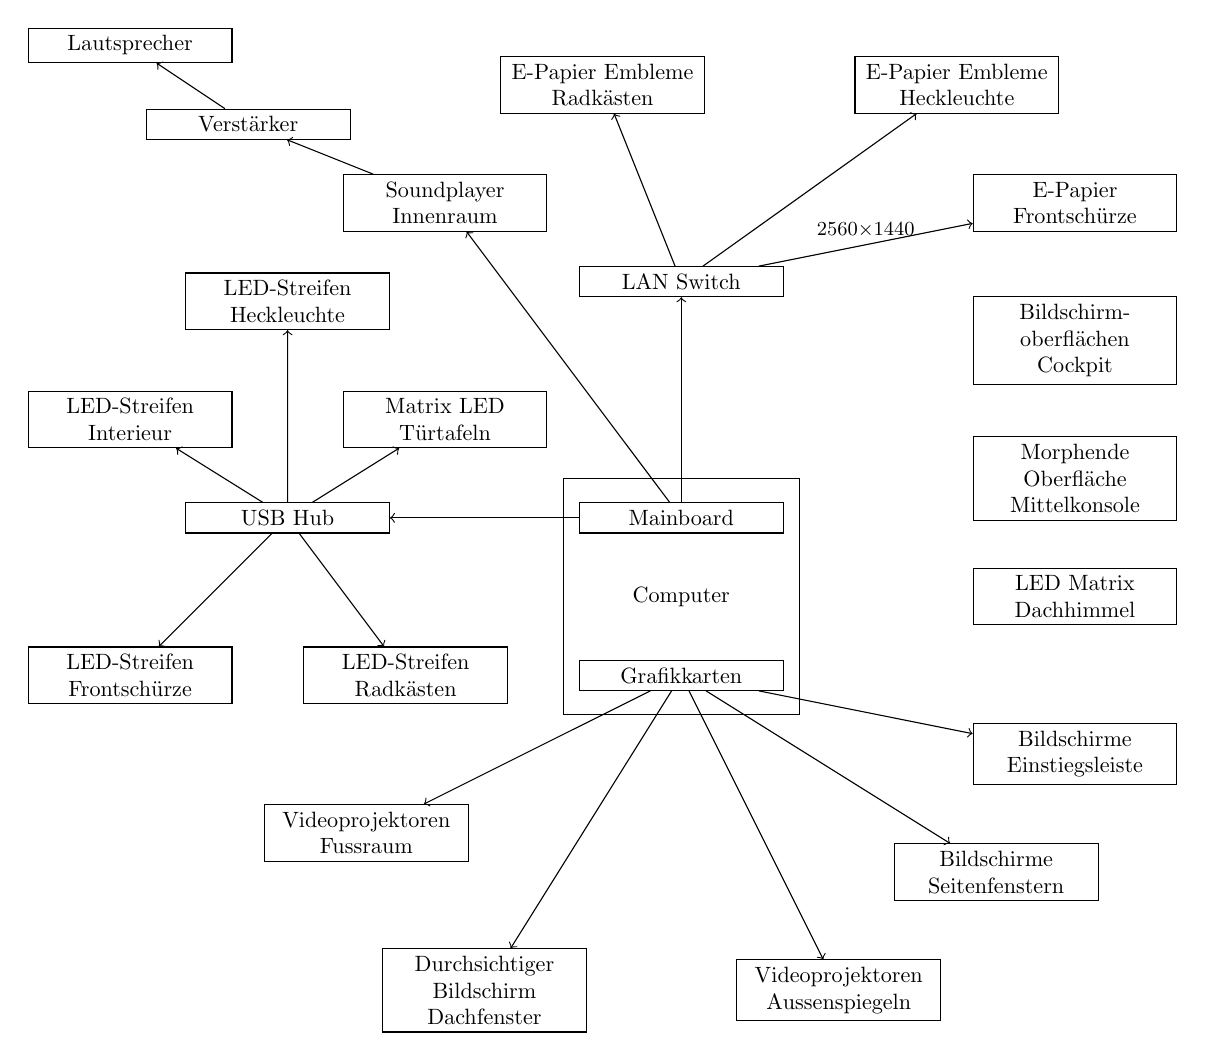
\begin{tikzpicture}[every node/.style={scale=0.8}]
	\node[text width=3.2cm, align=center] (Computer) at (0, -1) {Computer};
	\draw[draw=black] (-1.5,-2.5) rectangle ++(3,3);
	\node[draw, rectangle, text width=3cm, align=center] (Mainboard) at (0, 0) {Mainboard};
	\node[draw, rectangle, text width=3cm, align=center] (Grafikkarten) at (0, -2) {Grafikkarten};
	\node[draw, rectangle, text width=3cm, align=center] (LAN Switch) at (0, 3) {LAN Switch};
	\node[draw, rectangle, text width=3cm, align=center] (E-Papier Frontschürze) at (5, 4) {E-Papier Frontschürze};
	\node[draw, rectangle, text width=3cm, align=center] (LED-Streifen Frontschürze) at (-7, -2) {LED-Streifen Frontschürze};
	\node[draw, rectangle, text width=3cm, align=center] (E-Papier Embleme Radkästen) at (-1, 5.5) {E-Papier Embleme Radkästen};
	\node[draw, rectangle, text width=3cm, align=center] (LED-Streifen Radkästen) at (-3.5, -2) {LED-Streifen Radkästen};
	\node[draw, rectangle, text width=3cm, align=center] (Videoprojektoren Aussenspiegeln) at (2, -6) {Videoprojektoren Aussenspiegeln};
	\node[draw, rectangle, text width=3cm, align=center] (Bildschirme Seitenfenstern) at (4, -4.5) {Bildschirme Seitenfenstern};
	\node[draw, rectangle, text width=3cm, align=center] (LED-Streifen Heckleuchte) at (-5, 2.75) {LED-Streifen Heckleuchte};
	\node[draw, rectangle, text width=3cm, align=center] (E-Papier Embleme Heckleuchte) at (3.5, 5.5) {E-Papier Embleme Heckleuchte};
	\node[draw, rectangle, text width=3cm, align=center] (LED-Streifen Interieur) at (-7, 1.25) {LED-Streifen Interieur};
	\node[draw, rectangle, text width=3cm, align=center] (Matrix LED Türtafeln) at (-3, 1.25) {Matrix LED Türtafeln};
	\node[draw, rectangle, text width=3cm, align=center] (Bildschirme Einstiegsleiste) at (5, -3) {Bildschirme Einstiegsleiste};
	\node[draw, rectangle, text width=3cm, align=center] (Videoprojektoren Fussraum) at (-4, -4) {Videoprojektoren Fussraum};
	\node[draw, rectangle, text width=3cm, align=center] (Morphende Oberfläche Mittelkonsole) at (5, 0.5) {Morphende Oberfläche Mittelkonsole};
	\node[draw, rectangle, text width=3cm, align=center] (Durchsichtiger Bildschirm Dachfenster) at (-2.5, -6) {Durchsichtiger Bildschirm Dachfenster};
	\node[draw, rectangle, text width=3cm, align=center] (LED Matrix Dachhimmel) at (5, -1) {LED Matrix Dachhimmel};
	\node[draw, rectangle, text width=3cm, align=center] (Bildschirmoberflächen Cockpit) at (5, 2.25) {Bildschirm-oberflächen Cockpit};
	\node[draw, rectangle, text width=3cm, align=center] (Soundplayer Innenraum) at (-3, 4) {Soundplayer Innenraum};
	\node[draw, rectangle, text width=3cm, align=center] (USB Hub) at (-5, 0) {USB Hub};
	\node[draw, rectangle, text width=3cm, align=center] (Verstärker) at (-5.5, 5) {Verstärker};
	\node[draw, rectangle, text width=3cm, align=center] (Lautsprecher) at (-7, 6) {Lautsprecher};
	\draw[->] (Mainboard) -> (LAN Switch);
	\draw[->] (Mainboard) -> (Soundplayer Innenraum);
	\draw[->] (Mainboard) -> (USB Hub);
	\draw[->] (Grafikkarten) -> (Bildschirme Seitenfenstern);
	\draw[->] (Grafikkarten) -> (Bildschirme Einstiegsleiste);
	\draw[->] (Grafikkarten) -> (Videoprojektoren Fussraum);
	\draw[->] (Grafikkarten) -> (Videoprojektoren Aussenspiegeln);
	\draw[->] (Grafikkarten) -> (Durchsichtiger Bildschirm Dachfenster);
	\draw[->] (LAN Switch) -> node[above]{\small2560$ \times $1440} (E-Papier Frontschürze);
	\draw[->] (LAN Switch) -> (E-Papier Embleme Radkästen);
	\draw[->] (LAN Switch) -> (E-Papier Embleme Heckleuchte);
	\draw[->] (USB Hub) -> (LED-Streifen Frontschürze);
	\draw[->] (USB Hub) -> (LED-Streifen Radkästen);
	\draw[->] (USB Hub) -> (LED-Streifen Heckleuchte);
	\draw[->] (USB Hub) -> (LED-Streifen Interieur);
	\draw[->] (USB Hub) -> (Matrix LED Türtafeln);
	\draw[->] (Soundplayer Innenraum) -> (Verstärker);
	\draw[->] (Verstärker) -> (Lautsprecher);
\end{tikzpicture}
	\caption[Ansteuerung Komponenten im Prototypen]{Ansteuerung Komponenten im Prototypen}
	\label{fig:tikz_ansteuerung}
\end{figure}
%TODO Grafik umgestalten%